\section{Properties of Wigner distributions}
\label{app:wigner}

Here we present important properties of the phase-point operators and the Wigner distribution that are used throughout the paper.

\begin{proposition}\label{thm:aproperties}
    For any dimension $d$, the phase-point operators satisfy:
    \begin{enumerate}
        \item[(i)]\label{en:a1} Hermiticity and unitarity: $A_{\bmx}^\dagger = A_{\bmx} = A_{\bmx}^{-1}$;
	    \item[(ii)]\label{en:a2} Closure under transposition: $A_{(x, p)}^T = A_{(x, p)}$;
	    \item[(iii)]\label{en:a3} Unit trace for odd $d$: $\tr[A_{\bmx}] = 1$;
	    \item[(iv)]\label{en:a4} Completeness relation: $\sum_{\bmz \in \cal{P}_d} A_{\bmz} = d\id$;
	    \item[(i)]\label{en:a5} Orthogonality: $\tr[A_{\bmx}^\dagger A_{\bm{x'}}] = d \delta_{\bmx,\bm{x'}}$.
	\end{enumerate}
\end{proposition}
\begin{proof}
	All properties follow from the definition in~\cref{eq:ax} along with properties of the displacement operator $D_{\bmx}$ and can be found in the literature, e.g.~\cite{cit:veitch,Vourdas_2004,cit:gross3}
\end{proof}

\begin{proposition}\label{thm:wstate}
  The Wigner distribution of a state $\rho \in \cal{B}(\cal{H}_d)$ is
  \begin{enumerate}
    \item[(i)]\label{en:w1} Real valued: $\W{\rho} \in \mathbb{R}^{d^2}$;
    \item[(ii)]\label{en:w2} Normalised: $\sum_{\bmz \in \cal{P}_d} \W[\bmz]{\rho}=1$;
    \item[(iii)]\label{en:w3} Bounded: $\abs{\W[\bmx]{\rho}} \leq \frac{1}{d}$.
    \item[(iv)]\label{en:w4} Additive under mixing: \vspace{2pt}\\
    $\W[\bmx]{p\rho_1 + (1-p)\rho_2} = p\W[\bmx]{\rho_1} + (1-p)\W[\bmx]{\rho_2}$;
    \item[(v)]\label{en:w5} Multiplicative under tensor products: \vspace{2pt}\\
    $\W[\bmx_A \oplus \bmx_B]{\rho_A \otimes \rho_B} = \W[\bmx_A]{\rho_A}\W[\bmx_B]{\rho_B}$.
	\end{enumerate}
\end{proposition}
\begin{proof}
	Proof of all properties can be found in the literature~\cite{cit:veitch,Vourdas_2004,cit:gross3,Wang_2019} except for property (iii) which we prove here.
	
Let $\{\lambda_i\}_{i \in \mathbb{Z}_d}$ be the (non-negative) eigenvalues of $\rho$, summing to 1.
Let $\{\alpha_{\bmx,i}\}_{i \in \mathbb{Z}_d}$ be the eigenvalues of $A_{\bmx}$. For any $\bmx, \alpha_{\bmx,i} \in \{-1, 1\}$, due to the hermiticity and unitarity of the phase-point operators. 
Then,
\begin{align}
	\abs{W_{\rho}(\bmx)} &= \frac{1}{d}\abs{\tr[A_{\bmx} \rho]} \leq \frac{1}{d} \abs{\sum_i \alpha_{\bmx,i} \lambda_i} \nonumber\\ &\leq \frac{1}{d}\sum_i \lambda_i = \frac{1}{d}.
\end{align}
The first inequality follows from Theorem 1 of~\cite{cit:mirsky} for the trace of complex matrices, while the second is the Cauchy-Schwarz inequality.
\end{proof}

\begin{proposition}
    \label{thm:wchannel}
    The Wigner distribution of a $\cptp$ operation $\E: \cal{B}(\cal{H}_{d_A}) \mapsto \cal{B}(\cal{H}_{d_B})$ is
    \begin{enumerate}
        \item[(i)]\label{en:wo1} Real-valued: $\W{\E} \in \mathbb{R}^{d^2} \times \mathbb{R}^{d^2}$;
        \item[(ii)]\label{en:wo2} Normalised: $\sum_{\bmz \in \cal{P}_{d_B}} \W[\bmz|\bmx]{\E} = 1$ \\ 
        for any $\bmx \in \cal{P}_{d_A}$;
        \item[(iii)]\label{en:wo3} Bounded: $\abs{\W[\bmy|\bmx]{\E}} \leq \frac{d_A}{d_B}$;
	    \item[(iv)]\label{en:wo4} Transitive: $\W[\bmy]{\E(\rho)} = \sum_{\bmz \in \cal{P}_{d_A}} \W[\bmy|\bmz]{\E} \W[\bmz]{\rho}$ for any $\bmy \in \cal{P}_{d_B}$.
    \end{enumerate}
\end{proposition}
If $d_A = d_B$, and in particular if operation $\E$ maps a Hilbert space onto itself, then the stochasticity condition $\abs{\W[\bmy|\bmx]{\E}} \leq 1$ is satisfied.
\begin{proof}
	Proof of all properties are provided by Wang \textit{et al.}~\cite{Wang_2019} except for property (iii) which is a direct consequence of the definition of $\W{\E}$ and the corresponding property (iii) in~\cref{thm:wstate}.
\end{proof}

%%%%%%%%%%%%%%%%%%%%%%%%%%%%%%%%%%%%%%%%

\section{Properties of majorization}
\label{app:major}

% TO SWAP d --> r, REPLACE ALL \bmd, \bm{d}, d_i WITH \r

\subsection{Comments on monotones and fragements}
The development of any monotone $\M(\rho)$ for a magic theory $\R$ can be viewed abstractly as
\begin{equation}
\M : \mbox{(pre-order of states)} \mapsto \mbox{(total order of numbers).} \nonumber
\end{equation}
More precisely, within the theory we order magic states as $\rho_1 \succ \rho_2$ whenever there is an operation $\E \in \O$ such that $\E(\rho_1) = \rho_2$. In general many states will not be interconvertible in both directions, so this ordering is a pre-order in the sense that incomparable states exist. A magic monotone projects this pre-order of states onto the real number line, and, through this lens, any two states are directly comparable in terms of their mapped values $\M(\rho_1)$, $\M(\rho_2)$. Of course, the price is that the monotone provides only a necessary, but not sufficient, condition for the transformation $\rho_1 \rightarrow \rho_2$.

The restriction of a magic theory $\R$ to some fragment $\R_\sigma$ can now be interpreted as a generalisation of the magic monotone construction: instead of mapping the pre-order of states in $\R$ onto the number line, we instead map this pre-order onto \emph{a simpler pre-order of states}. Therefore, we are retaining more of the original parent theory, while working in a scenario that admits greater structure and simplicity. We can view this as a mapping $\P_\sigma: \R \rightarrow \R_\sigma$ that restricts to a sub-theory (a $\sigma$--fragment) of the parent theory $\R$. Thus,
\begin{equation}
\P_\sigma: \mbox{(pre-order)} \longrightarrow \mbox{(simpler pre-order).}
\end{equation}
By framing the projection onto a fragment in this light, we can view Theorem \ref{thm:frag} as a statement that the collection $\{\P_\sigma\}_{\sigma \in \F}$ provides a complete set of generalized monotones for the theory.
\subsection{Simple--majorization equivalence conditions}

In the unital fragment, namely the limit of infinite temperature, $\beta = 0$, the free state is the maximally mixed state $\frac{1}{n}\id$ with uniform Wigner distribution $\frac{1}{n}\bm{1} = (\frac{1}{n},\dots,\frac{1}{n})$.
This fragment is governed by simple majorization and we first prove strong equivalences for this type of majorization.
\begin{proposition}\label{prop:major}
Given $\bmx, \bmy \in \mathbb{R}^n$ the following statements are equivalent:
 \begin{enumerate}
	\item[(i)]\label{en:m1} $\bmx \prec \bmy$;
	\item[(ii)]\label{en:m2} $\bmx = B \bmy$ for bistochastic $B$;
	\item[(iii)]\label{en:m3} $\sum\limits_{i=1}^n \abs{x_i - t} \leq \sum\limits_{i=1}^n \abs{y_i - t}$ for all $t \in \mathbb{R}$;
	\item[(iv)]\label{en:m4} $\sum\limits_{i=1}^n (x_i - t)^+ \leq \sum\limits_{i=1}^n (y_i - t)^+$ for all $t \in \mathbb{R}$ and \vspace{5pt}\\ $\sum\limits_{i=1}^n x_i = \sum\limits_{i=1}^n y_i$, where $(x)^+ = \max{\{x, 0\}}$;
	\item[(v)]\label{en:m5} $L_{\bmx}(t) \leq L_{\bmy}(t)$ for $t\in [0,1)$	and \vspace{5pt}\\ $L_{\bmx}(1) = L_{\bmy}(1)$, where $L_{\bmz}(t) = L_{\bmz|\frac{1}{n}\bm{1}}(t)$.
 \end{enumerate}
\end{proposition}
	The equivalence between (i) and (ii) is the statement of the Hardy, Littlewood and Polya theorem and is taken as our definition of majorisation in the main text.
	
	The rest of the properties are well-known and proofs can be found in~\cite{cit:marshall,cit:bhatia,cit:nielsen,cit:lostaglio}.



\begin{lemma} Let $\p$ be a quasi-probability distribution and let $\r$ be a probability distribution with strictly non-zero components. Let $a > 0$ and $b \in \mathbb{R}$ then $L_{a\p + b \r | \r} (x) = a L_{\p |\r}(x) + b x$.
\end{lemma}\label{lemma:Lorenz_linearity}
\begin{proof} The Lorenz curve of $a\p + b \r$ relative to $\r$ passes through $(0,0)$ and the points $(\sum_{i=1}^k{r_{\pi(i)}}, \sum_{i=1}^k(a \p + b \r)_{\pi(i)})$ where $\pi$ is the permutation that puts $(a p_i/r_i + b)$ in non-increasing order. Since $a > 0$, the permutation $\pi$ puts  $(p_i/r_i)$ in non-increasing order too. We thus have
\begin{align*}
&\left( \sum_{i=1}^kr_{\pi(i)}, \sum_{i=1}^k(a \p + b \r)_{\pi(i)} \right) = \\ 
&\left( \sum_{i=1}^k r_{\pi(i)},a \sum_{i=1}^k  p_{\pi(i)} + b\sum_{i=1}^k r_{\pi(i)} \right) \nonumber,
\end{align*}
therefore the value of the Lorenz function at each potential elbow point $x_k = \sum_{i=1} ^kr_{\pi(i)}$ is given by
\begin{align}
&L_{a \p +b \r|\r} (x_k) = a L_{\p|\r} (x_k) + b L_{\r|\r}(x_k) = \nonumber\\
&a L_{\p|\r} (x_k) + b x_k,
\end{align}
so we have $L_{a\p  + b\r|\r} (x) = a L_{\p |\r}(x) + b x$ for any $x \in [0,1]$ due to linearity.
\end{proof}

\begin{lemma}\label{lem:lcmax}
	Given a magic state $\rho$, the maximum $L_\star$ of its Lorenz curve $\lc{\rho}{\sigma}(x)$ is independent of the $\sigma$--fragment and equal to $1+\sn{\rho}$. Moreover, the majorization constraint is stronger than mana in every fragment.
\end{lemma}
\begin{proof}
	We denote the Wigner distributions of the states compactly as vectors $\bmw(\rho) \equiv W_\rho(x)$ and $\bmw(\sigma) \equiv W_\sigma(x)$.
	We choose the component indexing so that the rescaled distribution 
	\begin{equation}
		\widetilde{\bmw}(\rho|\sigma) \coloneqq \left(\frac{w(\rho)_1}{w(\sigma)_1}, \dots, \frac{w(\rho)_{d^2}}{w(\sigma)_{d^2}} \right)^T,
	\end{equation}
	is sorted, $\widetilde{\bmw} = \widetilde{\bmw}^\downarrow$.
	Note that all components of $\bmw(\sigma)$ are positive, so $\widetilde{w}_i \geq 0$ if and only if $w(\rho)_i \geq 0$ for any $i=1,\dots,d^2$.
	
	Let $i_\star$ be the index of the smallest non-negative component of $\widetilde{\bmw}^\downarrow$.
	Then, $w(\rho)_i < 0$ if and only if $i > i_\star$, so the maximum of Lorenz curve $\lc{\rho}{\sigma}(x)$ takes the value 
	\begin{equation}
		\lc{\rho}{\sigma}(x_{i_\star}) = \sum_{i=1}^{i_\star} w(\rho)_i,
	\end{equation}
	and is achieved at
	\begin{equation}\label{eq:maxloc}
		x_{i_\star} \coloneqq \sum_{i=1}^{i_\star} w(\sigma)_i.
	\end{equation}

	The location of the maximum ($x=x_{i_\star}$) varies from fragment to fragment, but its value is independent of $\sigma$,
	\begin{align}
	L_\star &:=	\lc{\rho}{\sigma}(x_{i_\star}) 
		= \sum\limits_{\bmx: \W[\bmx]{\rho} \geq 0} \W[\bmx]{\rho} \nonumber \\
		&= 1 + \sn{\rho}.
	\end{align}
	
Since the magic monotone mana is a monotonic function of sum-negativity, $\rm{mana}(\rho) \coloneqq \ln{(2\hspace{1pt}\sn{\rho}+1)}$, we see that mana corresponds precisely to the peak of the Lorenz curve $L_{\rho|\sigma}(x)$. Therefore, mana is one of $d^{2n}$ constraints, so majorization is strictly a stronger constraint in any fragment.
\end{proof}


\subsection{Embedding map}

Any $\r$--majorization problem can be rephrased as a simple majorization problem in a higher dimensional space via the embedding map.
\begin{definition}
  The embedding map $\Gamma_{\r}:\mathbb{R}^n \mapsto \mathbb{R}^N, N = \sum\limits_{i=1}^n r_i$ is the function
  \begin{equation}
    \Gamma_{\r}(\bmw) = \bigoplus_{i=1}^n w_i\  \frac{1}{r_i}\bm{1},
  \end{equation}
where $\bm{1}/r_i$ is the $r_i$--dimensional uniform distribution.
The left inverse $\Gamma_{\r}^{-1}: \mathbb{R}^N \mapsto \mathbb{R}^n$ is defined to sum up the elements in each block of $\Gamma_{\r}(\bmw)$, so that
  \begin{equation}
     \Gamma_{\r}^{-1}(\oplus_{i=1}^n w_i \bm{1}/r_i) = \bmw.
  \end{equation}
  This is not a right inverse, because $\Gamma_{\r}$ is not surjective.
\end{definition}
The direct sum simply amounts to listing the uniform distributions one after the other.
The embedding map maps the Gibbs distribution to the uniform distribution, $\Gamma_{\r}(\r) = \bm{1}/N$.
Then, a non-increasing ordering $\Gamma_{\r}(\bmz)^\downarrow$ in the new space, corresponds to the so-called ``$\beta$-ordering'' of the original vector denoted by the permutation $\pi$ in~\cref{eq:lc}, mapping $(w_i/r_i) \mapsto (w_i/r_i)^\downarrow$ for all $i=1,\dots,n$.

\subsection{\textit{r}-majorization equivalence conditions}

We take the opportunity here	 to simply list useful equivalent statements for $\r$--majorisation.

\begin{proposition}\label{prop:rmajor}
Given $\bmx, \bmy, \r \in \mathbb{R}^n$, such that the components of $\r$ are positive, the following statements are equivalent:
  \begin{enumerate}
    \item[(i)] $\bmx \prec_{\r} \bmy$;
    \item[(ii)] $\Gamma_{\r}({\bmx}) \prec \Gamma_{\r}({\bmy})$;
    \item[(iii)]\label{en:tm3} $\sum\limits_{i=1}^n \abs{x_i - r_i t} \leq \sum\limits_{i=1}^n \abs{y_i - r_i t}$ for all $t \in \mathbb{R}$;
    \item[(iv)] $\sum\limits_{i=1}^n (x_i - r_i t)^+ \leq \sum\limits_{i=1}^n (y_i - r_i t)^+$ for all $t \in \mathbb{R}$ and \vspace{5pt}\\ $\sum\limits_{i=1}^n x_i = \sum\limits_{i=1}^n y_i$;
    \item[(v)] $L_{\bmx|\r}(t) \leq L_{\bmy|\r}(t)$ for $t\in [0,1)$ and \vspace{5pt}\\ $L_{\bmx|\r}(1) = L_{\bmy|\r}(1)$.
  \end{enumerate}
\end{proposition}
\begin{proof}$ $\vspace{-12pt}\\
\begin{enumerate}
	\item[1$\leftrightarrow2$]
	Suppose there exists a $\r$--stochastic $A$ such that $\bmx = A\bmy$ and let $B = \Gamma_{\r} \circ A \circ \Gamma_{\r}^{-1}$.
$B$ is a $N$--dimensional bistochastic matrix, since composition of stochastic matrices is stochastic and $(\Gamma_{\r} \circ A \circ \Gamma_{\r}^{-1})\big(\frac{1}{N}\bm{1}\big) = (\Gamma_{\r} \circ A) (\r) = \Gamma_{\r}(\r) = \frac{1}{N}\bm{1}$. Then, $B$ maps $\Gamma_{\r}({\bmy})$ to $\Gamma_{\r}({\bmx})$.

	Conversely, given $B$, let $A = \Gamma_{\r}^{-1} \circ B \circ \Gamma_{\r}$.
	Similarly, $A$ is a $\r$--stochastic matrix that maps $\bmy$ to $\bmx$.
	\item[$2\leftrightarrow3$] These \hspace{1pt} three \hspace{1pt} statements \hspace{1pt} are \hspace{1pt} equivalent \hspace{1pt} to \hspace{1pt} state-
	\item[$2\leftrightarrow4$] \vspace{-7pt} ments (iii), (iv), (v) \hspace{1pt} in~\cref{prop:major} respectively, 
	\item[$2\leftrightarrow5$] \vspace{-7pt} for the embedded vectors $\Gamma_{\r}({\bmx}), \Gamma_{\r}({\bmy})$, which becomes apparent by rewriting
	\begin{align*}
	&\hspace{15pt} \sum\limits_{i=1}^n \abs{x_i - r_i t} = \sum\limits_{i=1}^n r_i \abs{\frac{x_i}{r_i} - t} = \sum\limits_{i=1}^N \abs{\Gamma_{\r}(\bmx)_i - t}, \\[3pt]
	&\hspace{15pt} \sum\limits_{i=1}^n (x_i - r_i t)^+ = \sum\limits_{i=1}^N (\Gamma_{\r}(\bmx)_i - t)^+ \text{ and} \\[6pt]
	&\hspace{15pt} L_{\bmx|\r}(t) = L_{\Gamma_{\r}(\bmx)}(t),
	\end{align*} 
and similarly for the right hand sides of the inequalities.
\end{enumerate}
\vspace{-19pt}
\end{proof}

%%%%%%%%%%%%%%%%%%%%%%%%%%%%%%%%%%%%%%%%

\section{Technical properties of $\sigma$--fragments}
\label{app:frag}

In this section, we discuss some technical aspects of general $\sigma$--fragments.

\begin{proposition}\label{thm:frag_app}
    Let $\R_\sigma = (\O_\sigma, \F_\sigma)$ be a $\sigma$--fragment of magic theory $\R = (\O, \F)$. 
    The following statements hold:
    \begin{enumerate}
        \item No $\sigma$--fragment is empty.
        \item If a free operation leaves two states invariant, then it also leaves their mixtures invariant, 
        \begin{equation*}
            \O_{\sigma} \cap \O_{\sigma'} \subseteq \O_{p\sigma + (1-p)\sigma'}\ \text{for any}\ p \in [0,1].
        \end{equation*}
    \end{enumerate}
\end{proposition}
\begin{proof}$ $\vspace{-12pt}\\

\begin{enumerate}
    \item The identity channel $1_{\rm{C}}$ belongs to every $\sigma$--fragment, as $1_{\rm{C}} \in \O$ and $1_{\rm{C}}\sigma = \sigma$ for all $\sigma \in \F$.
    
    \item Let $\E \in \O_{\sigma} \cap \O_{\sigma'}$.
    Then $\E \in \cptp$ and corresponds to stochastic Wigner distribution $\W{\E}$ such that $\W{\E} \W{\sigma} = \W{\sigma}$ and $\W{\E} \W{\sigma'} = \W{\sigma'}$.
    Then, $\W{\E} \W{p\sigma + (1-p)\sigma'} = \W{p\sigma + (1-p)\sigma'}$ for any $p \in [0,1]$ due to the additive property~\ref{en:w4} of the Wigner distribution, implying that state $p\sigma + (1-p)\sigma'$ is also left invariant by $\E$.
\end{enumerate}
\vspace{-20pt}
\end{proof}

Any free state $\sigma \in \F$ corresponds to a $d^2$--dimensional probability distribution $\W{\sigma}$ and any free operation $\E \in \O$ corresponds to a $d^2 \times d^2$ stochastic matrix (or conditional probability distribution) $\W{\E}$.
Note that these mappings are one-to-one due to the orthogonality of the phase-point operators as an operator basis.

Note further that free states $\F$ are mapped onto a \emph{strict subset} of the set of probability distributions.
As a counterexample, the sharp $d^2$--dimensional probability distribution $(1, 0, \dots, 0)$ does not correspond to any qudit Wigner distribution because of the boundedness condition in~\cref{thm:wstate}.

Similarly, not all stochastic matrices correspond to completely positive operations.
As an example, consider the permutation matrix
\begin{equation}
    \Pi_X = \begin{psmallmatrix}
        0 & 1 & 0 & 0 & 0 \\
        0 & 0 & 0 & 0 & 1 \\
        0 & 0 & 0 & 1 & 0 \\
        1 & 0 & 0 & 0 & 0 \\
        0 & 0 & 1 & 0 & 0
    \end{psmallmatrix} \otimes \begin{psmallmatrix}
        0 & 0 & 1 & 0 & 0 \\
        0 & 0 & 0 & 0 & 1 \\
        0 & 0 & 0 & 1 & 0 \\
        1 & 0 & 0 & 0 & 0 \\
        0 & 1 & 0 & 0 & 0    
    \end{psmallmatrix} \in {\rm{S}}_5({\W{\frac{1}{5}\id}}).
\end{equation}
It preserves the uniform distribution $\W{\frac{1}{5}\id}$, but it does not correspond to any positive (hence quantum) operation.

We now prove a result on the independence of the Lorenz curve constraints.
\begin{proposition}\label{thm:elbows}
	Let $\rho, \tau$ be two quantum states with Lorenz curves $\lc{\rho}{\sigma}(x), \lc{\tau}{\sigma}(x)$ in the $\sigma$--fragment.
	
	Let $t$ be the number of elbows of $\lc{\tau}{\sigma}(x)$ at locations $x_1, \dots, x_t$.
	
	Then, $\lc{\rho}{\sigma}(x) \geq \lc{\tau}{\sigma}(x)$ for all $x \in [0,1]$ iff $\lc{\rho}{\sigma}(x_{i}) \geq \lc{\tau}{\sigma}(x_{i})$ for all $i =1,\dots,t$.
\end{proposition}
\begin{proof}	
	$\lc{\rho}{\sigma}(x) \geq \lc{\tau}{\sigma}(x)$ for all $x \in [0,1]$ trivially implies $\lc{\rho}{\sigma}(x_{i}) \geq \lc{\tau}{\sigma}(x_{i})$ for all $i = 1,\dots,n'$.
	
	Conversely, assume that $\lc{\rho}{\sigma}(x_{i}) \geq \lc{\tau}{\sigma}(x_{i})$ for all $i = 1,\dots,r$.
	First, let $x_0 = 0$ and $x_{n'+1} = 1$, so that $\lc{\rho}{\sigma}(x_0) = \lc{\tau}{\sigma}(x_0) = 0$ and $\lc{\rho}{\sigma}(x_{n'+1}) = \lc{\tau}{\sigma}(x_{n'+1}) = 1$.
	Hence, we can extend the set of elbows $E$ to $E' = E \cup \{x_0, x_{n'+1}\}$.
	
	Pick two consecutive locations $x_{i}, x_{i+1}$ in $E'$ and consider the line segment $\ell_\tau(x)$ connecting points $(x_{i}, \lc{\tau}{\sigma}(x_{i}))$ and $(x_{i+1}, \lc{\tau}{\sigma}(x_{i+1}))$ as well as the line segment $\ell_\rho(x)$ connecting points $(x_{i}, \lc{\rho}{\sigma}(x_{i}))$ and $(x_{i+1}, \lc{\rho}{\sigma}(x_{i+1}))$.
	This is illustrated in~\cref{fig:elbows_proof}.
\begin{figure}[h]
    \centering
    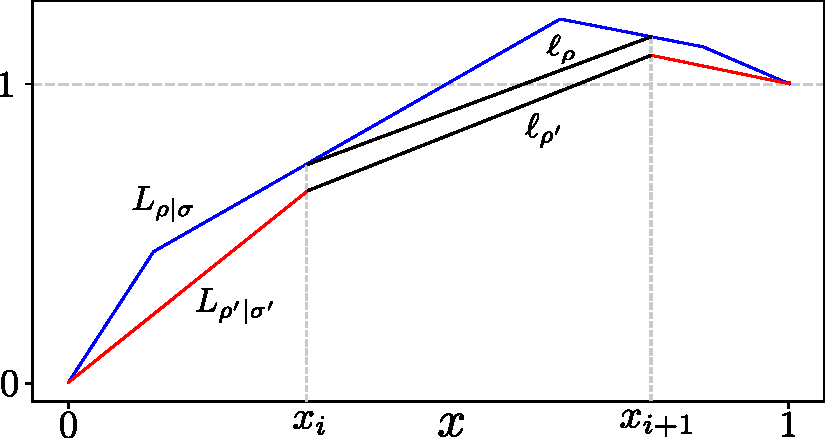
\includegraphics[scale=0.6]{figs/elbows_proof.pdf}
    \caption{\textbf{Illustration of~\cref{thm:elbows}}.
    }
    \label{fig:elbows_proof}
\end{figure}

	Due to concavity of $\lc{\rho}{\sigma}$, it is clear that for all $x \in [x_{i}, x_{i+1}]$, we have $\lc{\rho}{\sigma}(x) \geq \ell_\rho(x) \geq \ell_\tau(x) = \lc{\tau}{\sigma}(x)$.
	This argument can be made in all intervals $[x_{i}, x_{i+1}]$ with $i=0,\dots,n'$, so the proof is complete.
\end{proof}
This theorem is of practical importance in reducing the necessary distillation constraints derived via majorization in $\sigma$--fragments.

%%%%%%%%%%%%%%%%%%%%%%%%%%%%%%%%%%%%%%%%

\section{Lorenz curves in the unital fragment}
\label{app:lcsu_technical}

\subsection{Binomial distributions and error bounds}\label{app:phi}
Consider an experiment consisting of $n$ trials of throwing a $p$--coin, that is a coin with probability $p$ of landing on one side and $1-p$ of landing on the other.
We express the sums over an even number $m$ of successful trials $\Phi_+$ and an odd number $m$ of successful trials $\Phi_-$,
\begin{align}	
	\Phi_+(m; n, p) &\coloneqq \sum\limits_{\ell=0}^{m/2} \binom{n}{2\ell} p^{2\ell} (1-p)^{n-2\ell}, \nonumber\\ 
	&\text{for even integers } m\in[0,n], \label{eq:fp_app} \\
	\Phi_-(m; n, p) &\coloneqq \sum\limits_{\ell=1}^{(m-1)/2} \binom{n}{2\ell+1} p^{2\ell+1} (1-p)^{n-(2\ell+1)}, \nonumber\\ 
	&\text{for odd integers }m\in[0,n]. \label{eq:fn_app}
\end{align}
Note that index $m$ only takes even (odd) values when labelling $\Phi_+$ ($\Phi_-$).
In~\cref{app:lcsu_coord}, we will use $\Phi_+$ and $\Phi_-$ to express the elbow coordinates of Lorenz curves in the unital fragment.

We also define the classical entropy of a $p$--coin and the classical relative entropy between a $p$--coin and a $q$--coin,
\begin{align}
	S(p) &\coloneqq -p\log{p} -(1-p)\log{(1-p)}, \label{eq:ent}\\
	\ent{p}{q} &\coloneqq p \log{\frac{p}{q}} + (1-p) \log{\frac{1-p}{1-q}}. \label{eq:ent_rel}
\end{align}
They are symmetric in the sense that $S(p) = S(1-p)$ and $\ent{p}{q} = \ent{1-p}{1-q}$.

A useful result is the entropic bound on a combination~\cite{cit:ash}.
\begin{lemma}\label{lem:comb_bounds}
	For all $\ell\in [1,n-1]$,
	\begin{align}
		&\left[ 8\ell\left(1-\frac{\ell}{n}\right) \right]^{-\frac{1}{2}} 2^{n S\left(\frac{\ell}{n}\right)} \leq \binom{n}{\ell} \leq \\
		&\left[ 2\pi \ell\left(1-\frac{\ell}{n}\right) \right]^{-\frac{1}{2}} 2^{n S\left(\frac{\ell}{n}\right)}.
	\end{align}
\end{lemma}
The proof provided in~\cite{cit:ash} proceedx with direct calculation for the edge cases $\ell = 1,2, n-1, n-2$ and use Stirling's approximation for the remaining cases.

With the help of this lemma, we directly arrive at 
\begin{theorem}\label{thm:bounds_strict}
	Given fixed positive integer $n$ and probability $p$, $\Phi_+, \Phi_-$ satisfy the following bounds:
	\begin{align*}
		\begin{split}
		&\text{1. } \Phi_+(m; n, p) \geq \sum\limits_{\ell=0}^{m/2}\left[ 16\ell\left(1-\frac{2\ell}{n}\right) \right]^{-\frac{1}{2}} 2^{-n\ent{\frac{2\ell}{n}}{p}}, \\
		&\hspace{14pt} \text{for all even } m\in [2,n] \\
		&\text{2. } \Phi_+(m; n, p) \leq \sum\limits_{\ell=0}^{m/2}\left[ 4\pi\ell\left(1-\frac{2\ell}{n}\right) \right]^{-\frac{1}{2}} 2^{-n\ent{\frac{2\ell}{n}}{p}}, \\
		&\hspace{14pt} \text{for all even } a\in [2,n] \\
		&\text{3. } \Phi_-(m; n, p) \geq \sum\limits_{\ell=1}^{(m-1)/2}\left[ 16(\ell+1)\left(1-\frac{2\ell+1}{n}\right) \right]^{-\frac{1}{2}} \times \\
		&\hspace{14pt} \times 2^{-n\ent{\frac{2\ell+1}{n}}{p}},\ \text{for all odd }a\in [1,n] \\
		&\text{4. } \Phi_-(m; n, p) \leq \sum\limits_{\ell=1}^{(m-1)/2}\left[ 4\pi(\ell+1)\left(1-\frac{2\ell+1}{n}\right) \right]^{-\frac{1}{2}} \times \\
		&\hspace{14pt} \times 2^{-n\ent{\frac{2\ell+1}{n}}{p}},\ \text{for all odd } a\in [1,n]
		\end{split}
	\end{align*}
\end{theorem}
\begin{proof}
	All four statements follow from application of~\cref{lem:comb_bounds} on the combinatorial coefficient and the defintion of relative entropy given in~\cref{eq:ent_rel}
\end{proof}

\subsection{Lorenz curve coordinates in the unital fragment}\label{app:lcsu_coord}
The Wigner distribution of the $n$--copy qutrit maximally mixed state $\left(\id/3\right)^{\otimes n}$ is the uniform probability distribution over the phase space, consisting of $9^n$ components equal to $9^{-n}$.
The Wigner distribution of the 1-copy $\epsilon$--noisy Strange state $\rho_{\rm{S}}(\epsilon)$ in the unital fragment consists of some permutation of a single negative component
\begin{equation}
	- v(\epsilon) \coloneqq - \left( \frac{1}{3} -\frac{4}{9}\epsilon \right),
\end{equation} 
and $8$ positive components
\begin{equation}
	u(\epsilon) \coloneqq \frac{1}{6} -\frac{1}{18}\epsilon.
\end{equation}
where in the unital fragment we need the condition $0 \leq \epsilon < 3/4$, so that the state contains some Wigner negativity ($-v < 0$).
It is also clear that $v \geq u$ in the interval $0 \leq \epsilon \leq 3/7$, while $u > v$ in the interval $3/7 < \epsilon < 3/4$.

The Wigner distribution of the $n$--copy $\epsilon$--noisy Strange state $\rho_{\rm{S}}(\epsilon)^{\otimes n}$ in the unital fragment is given by the convolution $\W{\rho_{\rm{S}}(\epsilon)^{\otimes n}} = W_{\rho_{\rm{S}}(\epsilon)}^{\otimes n}$.
In general, $\rho_{\rm{S}}(\epsilon)^{\otimes n}$ contains $n + 1$ distinct components, labelled $0,\dots, n$.
We present the distinct Wigner components of $\rho_{\rm{S}}(\epsilon)^{\otimes n}$ along with their multiplicites in~\cref{tab:lcsu}.
Note that LHS (RHS) refers to elbow coordinates $i$ on the left of and including (right of) the Lorenz curve maximum, stated precisely as
\begin{align}
&\text{LHS: } 0 \leq i \leq \left\lfloor \frac{n}{2} \right\rfloor \text{ and} \\
&\text{RHS: } \left\lfloor \frac{n}{2} \right\rfloor +1 \leq i \leq n.
\end{align}
\begin{table}[h]
  \def\arraystretch{1.5}
  \centering
  \begin{tabular}{c|c|c|r|r}
    \multicolumn{3}{c|}{Case} & \multicolumn{1}{c}{$m_{i}(n, \epsilon)$} & \multicolumn{1}{|c}{$w_{i}(n, \epsilon)$} \\[0.5ex]\hline
    \multirow{4}{*}{\raisebox{-4ex}{\rotatebox[origin=c]{90}{$0\leq \epsilon < \frac{3}{7}$}}} & \hspace{0.8ex}\multirow{2}{*}{\raisebox{-1ex}{\rotatebox[origin=c]{90}{$n$ even}}}\hspace{0.8ex} & LHS & $8^{2i}\binom{n}{2i}$ & $\left( \frac{1}{6} - \frac{1}{18}\epsilon \right)^{2i}\left( -\frac{1}{3} + \frac{4}{9}\epsilon \right)^{n-2i}$ \\
    & & RHS & $8^{n-2i}\binom{n}{2i}$ & $\left( \frac{1}{6} - \frac{1}{18}\epsilon \right)^{n-2i}\left( -\frac{1}{3} + \frac{4}{9}\epsilon \right)^{2i}$ \\ \cline{2-5}
    & \multirow{2}{*}{\raisebox{-2ex}{\rotatebox[origin=c]{90}{$n$ odd}}} & LHS & $8^{2i+1}\binom{n}{2i+1}$ & $\left( \frac{1}{6} - \frac{1}{18}\epsilon \right)^{2i+1}\left( -\frac{1}{3} + \frac{4}{9}\epsilon \right)^{n-2i-1}$ \\
    & & RHS & $8^{n-2i-1}\binom{n}{2i+1}$ & $\left( \frac{1}{6} - \frac{1}{18}\epsilon \right)^{n-2i-1}\left( -\frac{1}{3} + \frac{4}{9}\epsilon \right)^{2i+1}$ \\ \hline
    \multirow{4}{*}{\raisebox{-4ex}{\rotatebox[origin=c]{90}{$\frac{3}{7}\leq \epsilon < \frac{3}{4}$}}} & \multirow{2}{*}{\raisebox{-1ex}{\rotatebox[origin=c]{90}{$n$ even}}} & LHS & $8^{n-2i}\binom{n}{2i}$ & $\left( \frac{1}{6} - \frac{1}{18}\epsilon \right)^{n-2i}\left( -\frac{1}{3} + \frac{4}{9}\epsilon \right)^{2i}$ \\
    & & RHS & $8^{2i}\binom{n}{2i}$ & $\left( \frac{1}{6} - \frac{1}{18}\epsilon \right)^{2i}\left( -\frac{1}{3} + \frac{4}{9}\epsilon \right)^{n-2i}$ \\ \cline{2-5}
    & \multirow{2}{*}{\raisebox{-2ex}{\rotatebox[origin=c]{90}{$n$ odd}}} & LHS & $8^{n-2i}\binom{n}{2i}$ & $\left( \frac{1}{6} - \frac{1}{18}\epsilon \right)^{n-2i}\left( -\frac{1}{3} + \frac{4}{9}\epsilon \right)^{2i}$ \\
    & & RHS & $8^{2i}\binom{n}{2i}$ & $\left( \frac{1}{6} - \frac{1}{18}\epsilon \right)^{2i}\left( -\frac{1}{3} + \frac{4}{9}\epsilon \right)^{n-2i}$ \\ \hline
  \end{tabular}
  \caption{Wigner components $w_{i}(n, \epsilon)$ of $\rho_{\rm{S}}(\epsilon)^{\otimes n}$ along with their multiplicities $m_{i}(n, \epsilon)$, with $0 \leq i \leq n$.
  The expressions change depending on the noise level $\epsilon$, the parity of the number of copies $n$ and whether the index $i$ is lower or higher than the index of the Lorenz curve maximum (LHS vs RHS).
  Multiplication $2i$ is considered modulo $(n+1)$.}
  \label{tab:lcsu}
\end{table}

Every Lorenz curve in the unital fragment contains $n$ elbows, which, along with the boundary points $(x_{-1}, L_{-1}) = (0,0)$ and $(x_{n}, L_{n}) = (1,1)$, are labelled by 
\begin{equation*}
\{(x_{i}, L_{i})\}_{i=-1,0,\dots,n}.
\end{equation*}
The maximum is the $\lfloor n/2 \rfloor$-th elbow and its coordinates are calculated by collecting all the positive Wigner components,
\begin{align}
	x_{\lfloor n/2 \rfloor} &= \frac{1}{2}\left(1 + \left(\frac{7}{9}\right)^n\right), \\
	L_{\lfloor n/2 \rfloor} &= \frac{1}{2}\left (1 + \left(\frac{15 - 8\epsilon}{9}\right)^n \right).
\end{align}
%\sum_{j: even}^n a^j \binom{n}{j} = \frac{1}{2} [ (1+a)^n + (1-a)^n ]

Expressions for all the elbow coordinates follow from summing up the Wigner components in decreasing order.
In~\cref{tab:lcsu_coord_elb_app}, we present the elbow coordinates of the $n$-copy, $\epsilon$--noisy Strange state Lorenz curve in the unital fragment for any combination of parameters $n, \epsilon$.
\begin{table}[h]
  \def\arraystretch{1.5}
  \centering
  \begin{tabular}{c|c|c|r|r}
\multicolumn{3}{c|}{\multirow{2}{*}{Case}} & \multicolumn{1}{c|}{$x_{i}$} & \multicolumn{1}{c}{$L_{i}$} \\
    \multicolumn{3}{c|}{} & \multicolumn{1}{c|}{$x_{i} - x_{\lfloor n/2 \rfloor}$} & \multicolumn{1}{c}{$L_{i} - L_{\lfloor n/2 \rfloor}$} \\[0.5ex]\hline 
    \multirow{4}{*}{\raisebox{-5ex}{\rotatebox[origin=c]{90}{$0\leq \epsilon < \frac{3}{7}$}}} & \hspace{0.8ex}\multirow{2}{*}{\raisebox{-3ex}{\rotatebox[origin=c]{90}{$n$ even}}}\hspace{0.8ex} & LHS & $\Phi_+\left(2i;n,\frac{8}{9}\right)$ & $\left( \frac{5}{3} - \frac{8}{9}\epsilon\ \right)^n \Phi_+\left(2i;n,\frac{12-4\epsilon}{15-8\epsilon}\right)$ \\
    & & RHS & $\Phi_-\left(2i;n,\frac{1}{9}\right)$ & $- \left( \frac{5}{3} - \frac{8}{9}\epsilon\ \right)^n\Phi_-\left(2i;n,\frac{3-4\epsilon}{15-8\epsilon}\right)$ \\ \cline{2-5}
    & \multirow{2}{*}{\raisebox{-3ex}{\rotatebox[origin=c]{90}{$n$ odd}}} & LHS & $\Phi_-\left(2i;n,\frac{8}{9}\right)$ & $\left( \frac{5}{3} - \frac{8}{9}\epsilon\ \right)^n \Phi_-\left(2i;n,\frac{12-4\epsilon}{15-8\epsilon}\right)$ \\
    & & RHS & $\Phi_-\left(2i;n,\frac{1}{9}\right)$ & $- \left( \frac{5}{3} - \frac{8}{9}\epsilon\ \right)^n\Phi_-\left(2i;n,\frac{3-4\epsilon}{15-8\epsilon}\right)$ \\ \hline
    \multirow{4}{*}{\raisebox{-5ex}{\rotatebox[origin=c]{90}{$\frac{3}{7}\leq \epsilon < \frac{3}{4}$}}} & \multirow{2}{*}{\raisebox{-3ex}{\rotatebox[origin=c]{90}{$n$ even}}} & LHS & $\Phi_+\left(2i;n,\frac{1}{9}\right)$ & $\left( \frac{5}{3} - \frac{8}{9}\epsilon\ \right)^n \Phi_+\left(2i;n,\frac{3-4\epsilon}{15-8\epsilon}\right)$ \\
    & & RHS & $\Phi_-\left(2i;n,\frac{8}{9}\right)$ & $- \left( \frac{5}{3} - \frac{8}{9}\epsilon\ \right)^n\Phi_-\left(2i;n,\frac{12-4\epsilon}{15-8\epsilon}\right)$ \\ \cline{2-5}
    & \multirow{2}{*}{\raisebox{-3ex}{\rotatebox[origin=c]{90}{$n$ odd}}} & LHS & $\Phi_+\left(2i;n,\frac{1}{9}\right)$ & $\left( \frac{5}{3} - \frac{8}{9}\epsilon\ \right)^n \Phi_+\left(2i;n,\frac{3-4\epsilon}{15-8\epsilon}\right)$ \\
    & & RHS & $\Phi_+\left(2i;n,\frac{8}{9}\right)$ & $- \left( \frac{5}{3} - \frac{8}{9}\epsilon\ \right)^n\Phi_+\left(2i;n,\frac{12-4\epsilon}{15-8\epsilon}\right)$ \\ \hline
  \end{tabular}
  \caption{Lorenz curve elbow coordinates in the unital fragment.
  The coordinate expressions depend on the noise level $\epsilon$, the parity of the number of copies $n$ and the location of the elbow relative to the maximum (LHS vs RHS).
  Multiplication $2i$ is considered modulo $(n+1)$.
  For completeness, note that $(x_{-1}, L_{-1}) \coloneqq (0,0)$ is not included in the table.
  }
  \label{tab:lcsu_coord_elb_app}
\end{table}

We can get explicit expressions for all $9^{n}$ points of the Lorenz curve $\lc{\rho_{\rm{S}}(\epsilon)^{\otimes n}}{(\id/3)^{\otimes n}}$, in terms of the elbow coordinates:
\begin{align}
    x_{ij} &= \left( 1-\frac{j}{m_{i}} \right) x_{i-1} + \frac{j}{m_{i}} x_{i}, \label{eq:x}\\
    L_{ij} &= \left( 1-\frac{j}{m_{i}} \right) L_{i-1} + \frac{j}{m_{i}} L_{i} \label{eq:l}
\end{align}
for $j = 1,\dots,m_{i}$ and $i=0,\dots,n$, where multiplicities $m_i = m_i(n, \epsilon)$ are given in~\cref{tab:lcsu}.

Consider the state 
\begin{equation*}
\rho_{\rm{S}}(\epsilon')^{\otimes n'} \otimes \left( \frac{1}{3}\id \right)^{\otimes (n-n')},
\end{equation*}
where tensoring with the maximally mixed state keeps the Lorenz curve unchanged, but increases the resolution of (the uniformly distributed) points.
The new point coordinates are given by:
\begin{align}
    &x_{ijk} = \left( 1-p_{ijk}\right) x_{i-1} + p_{ijk} x_{i} \label{eq:lcsu_xcoord}\\
    &L_{ijk} = \left( 1-p_{ijk} \right) L_{i-1} + p_{ijk} L_{i}, \label{eq:lcsu_lcoord}\\
    &\text{where } p_{ijk} = \frac{k + (j-1)9^{n-n'}}{9^{n-n'} m_{i}} \nonumber\\
    &\text{for } i=0,\dots,n',\ j = 1,\dots,m_{i}(n', \epsilon') \text{ and } k = 1,\dots,9^{n-n'}. \nonumber
\end{align}

We can unify the indices, by introducing a single index
\begin{equation}
    I(i,j,k) \coloneqq k + \left[ (j-1) + \sum_{\ell=0}^{i-1} m_{\ell}(n', \epsilon') \right]9^{n-n'},
\end{equation}
so that $I=1,2,\dots, 9^{n}$.
The elbow coordinates correspond to 
\begin{equation}
	I(i, m_{i}(n', \epsilon'), 9^{n-n'}) = \sum_{\ell=0}^{i} m_{\ell}(n', \epsilon'),\ i= 0,\dots,n'.
\end{equation}
The index function $I$ is bijective, i.e.
\begin{equation}
	(i,j,k) = (i',j',k') \Leftrightarrow I(i,j,k) = I(i',j',k').
\end{equation}

%%%%%%%%%%%%%%%%%%%%%%%%%%%%%%%%%%%%%%%%

\section{Technical details of the derivation of distillation bounds}
\label{app:lcst_technical}

\subsection{First and last elbow constraints}
\label{app:elb_constraints}
Here we prove two simple majorization constraints, one arising by considering only the ascending part of the Lorenz curves between the origin $(0,0)$ and the first elbow and the other by considering only the descending part of the curves between the last elbow and the endpoint $(1,1)$.
\begin{proposition}\label{prop:first_elb}
	Consider a magic state process $\rho \longrightarrow \tau$ with input and output Lorenz curves $\lc{\rho}{\sigma}(x), \lc{\tau}{\sigma}(x)$ in $\R_\sigma$ and denote by $X_0, X'_0$ the first elbow locations of the input and output curves respectively.
	
	Then, given any coordinates $(x_0, L_0)$ and $(x'_0, L'_0)$ on the input and output Lorenz curves, where $x_0 \leq X_0$ and $x'_0 \leq X'_0$, the process is possible in $\R_\sigma$ only if
\begin{equation}\label{eq:first_elb_bound1}
	\frac{L_0}{x_0} \geq \frac{L_0'}{x_0'}.
\end{equation}
\end{proposition}
\begin{proof}
Since both pairs of coordinates are located between $(0,0)$ and the first elbow of their respective curves, we can derive the bound via a simple interpolation on the line segment connecting the origin and the appropriate first elbow.

First assume that $x_0 < x'_0$ and consider the Lorenz curve constraint at $x = x_0$,
\begin{equation}
	\lc{\rho}{\sigma}(x_0) \geq \lc{\tau}{\sigma}(x_0).
\end{equation}
We can find the output state Lorenz curve coordinate $L'_\star$ at location $x = x_0$ by interpolating between the origin and the output state's first elbow, 
\begin{equation}
	L'_\star = \frac{x_0}{x'_0}L'_0.
\end{equation}
The process is then possible only if $L_0 \geq L_\star'$ which is a rearrangement of~\cref{eq:first_elb_bound1}.

If instead, $x_0 \geq x'_0$, consider the Lorenz curve constraint at $x = x'_0$,
\begin{equation}
	\lc{\rho}{\sigma}(x'_0) \geq \lc{\tau}{\sigma}(x'_0).
\end{equation}
We now need to find the input state Lorenz curve coordinate $L_\star$ at location $x = x'_0$ by interpolating between the origin and the input state's first elbow, 
\begin{equation}
	L_\star = \frac{x'_0}{x_0}L_0.
\end{equation}
The process is then possible only if $L_\star \geq L'_0$ which is again a rearrangement of~\cref{eq:first_elb_bound1}.
\end{proof}

\begin{proposition}\label{prop:last_elb}
	Consider a magic state process $\rho \longrightarrow \tau$ with input and output Lorenz curves $\lc{\rho}{\sigma}(x), \lc{\tau}{\sigma}(x)$ in $\R_\sigma$ and denote by $X_E, X'_E$ the last elbow locations of the input and output curves respectively.
	
	Then, given any coordinates $(x_E, L_E)$ and $(x'_E, L'_E)$ on the input and output Lorenz curves, where $x_E \geq X_E$ and $x'_E \geq X'_E$, the process is possible in $\R_\sigma$ only if
\begin{equation}\label{eq:last_elb_bound1}
	\frac{L_E - 1}{1-x_E} \geq \frac{L'_E - 1}{1-x_E'}.
\end{equation}
\end{proposition}
\begin{proof}
Since both pairs of coordinates are located between the last elbow of their respective curves and $(1,1)$, we can derive the bound via a simple interpolation on the line segment connecting the endpoint and the appropriate last elbow.

First assume that $x_E > x'_E$ and consider the Lorenz curve constraint at $x = x_E$,
\begin{equation}
	\lc{\rho}{\sigma}(x_E) \geq \lc{\tau}{\sigma}(x_E).
\end{equation} 
We can find the output state Lorenz curve coordinate $L'_\star$ at location $x = x_E$ by interpolating between the endpoint $(1,1)$ and the output state's last elbow, 
\begin{equation}
	L'_\star = 1 + \frac{1-x_E}{1-x'_E} (L'_E - 1)
\end{equation}
The process is then possible only if $L_E \geq L_\star'$ which is a rearrangement of~\cref{eq:last_elb_bound1}.

If instead, $x_E \leq x'_E$, consider the Lorenz curve constraint at $x = x'_E$,
\begin{equation}
	\lc{\rho}{\sigma}(x'_E) \geq \lc{\tau}{\sigma}(x'_E).
\end{equation} 
We now need to find the input state Lorenz curve coordinate $L_\star$ at location $x = x'_E$ by interpolating between the endpoint $(1,1)$ and the input state's last elbow, 
\begin{equation}
	L_\star = 1 + \frac{1-x'_E}{1-x_E} (L_E - 1).
\end{equation}
The process is then possible only if $L_\star \geq L'_E$ which is again a rearrangement of~\cref{eq:last_elb_bound1}.
\end{proof}

\subsection{Component-multiplicity pairs}
\label{app:cmpairs}
In general, a $1$--copy $d$--dimensional state $\rho$ is described exactly by its $d^2$--dimensional Wigner distribution $\W{\rho}$. 
The distribution $\W{\rho}$ is usually defined on the phase space, but it can be convenient to define it using pure vector notation. 
In particular, we introduce a component vector $\bmw(\rho) = (w_i)_{i=1,\dots,D}$ and a multiplicity vector $\bmm(\rho) = (m_i)_{i=1,\dots,D}$, where $D \leq d^2$ which together form a set of component-multiplicity pairs $\{(w_i, m_i)\}_{i=1,\dots,D}$.
\begin{definition}
	Consider a distribution $W$ and a positive integer $D \leq {\rm{dim}}\hspace{1pt}W$. 
	We call the set of ordered pairs $\{(w_i, m_i)\}_{i=1,\dots,D}$ a \emph{complete set of component-multiplicity pairs}, if $W$ contains $m_i$ components $w_i$ and $\sum_{i=0}^D m_i = d^2$.
\end{definition}
Therefore, such a set describes each component of $\W{\rho}$ exactly once.
As an example, two complete sets of pairs for the Strange state are $\{( -1/3, 1), ( 1/6, 8)\}$ and $\{(-1/3, 1), (1/6, 2), (1/6, 3), (1/6, 3)\}$.
The latter corresponds to the phase space split in~\cref{fig:pd_split}

Consider two states $\rho_A, \rho_B$ with Wigner distributions $\W{\rho_A}, \W{\rho_B}$ described respectively by complete sets of component-multiplicity pairs 
\begin{equation}
	\{(w_i, m_i)\}_{i=1,\dots,D_A} \text{ and } \{(w_j', m_j')\}_{j=0,\dots,D_B}.
\end{equation}
The multiplicative property of the Wigner distribution over a composite phase space $\cal{P}_{d_A} \times \cal{P}_{d_B}$ shown in~\cref{thm:wstate},
\begin{equation}
	\W[\bmx_A \oplus \bmx_B]{\rho_A \otimes \rho_B} = \W[\bmx_A]{\rho_A}\W[\bmx_B]{\rho_B},
\end{equation}
implies that the distribution $\W{\rho_A \otimes \rho_B}$ is $d_A^2 d_B^2$--dimensional and contains components of the form $w_i w_j'$. 
Therefore, the set $\{(w_i w_j', m_i m_j')\}$ with $i=1,\dots,D_A$ and $j=1,\dots,D_B$ is a complete set of component-multiplicity pairs for the distribution of the composite system $\W{\rho_A \otimes \rho_B}$.
This is true because all components are of the form $w_i w_j'$ and 
\begin{equation*}
	\sum_{i=1}^{D_A}\sum_{j=1}^{D_B} m_i m_j' = \sum_{i=1}^{D_A} m_i \sum_{j=1}^{D_B} m_j' = d_A^2 d_B^2.
\end{equation*}

Note that the rescaled distribution is also multiplicative,
\begin{align}
	&\widetilde{\rm{W}}_{\rho_A \otimes \rho_B | \gamma_A \otimes \gamma_B}(\bmx_A \oplus \bmx_B) = \frac{\W[\bmx_A \oplus \bmx_B]{\rho_A \otimes \rho_B}}{\W[\bmx_A \oplus \bmx_B]{\gamma_A \otimes \gamma_B}} = \nonumber \\
	&\frac{\W[\bmx_A]{\rho_A}\W[\bmx_B]{\rho_B}}{\W[\bmx_A]{\gamma_A}\W[\bmx_B]{\gamma_B}} = \widetilde{\rm{W}}_{\rho_A | \gamma_A}(\bmx_A)\widetilde{\rm{W}}_{\rho_B  | \gamma_B}(\bmx_B),
\end{align}
so a complete set of component-multiplicity pairs can be obtained for this distribution in the same fashion as for usual Wigner distributions.

Given a state $\rho$ and a complete set of component-multiplicity pairs describing its Wigner distribution $\W{\rho}$, we now provide a method of computing the components (and multiplicities) of the $n$--copy distribution $\W{\rho}^{\otimes n}$.
\begin{lemma}\label{lem:ncopycomponents}
	Let $W$ be a distribution defined by a complete set of component-multiplicity pairs $\{(w_i, m_i)\}_{i=1,\dots,D}$ with $D \leq {\rm{dim}}\hspace{1pt}W$ and consider the distribution $W^{\otimes n}$ obtained by taking the $n$-fold (Kronecker) product $W \otimes \dots \otimes W$ between $n$ copies of $W$.
	
	Denote by $C_D^n \coloneqq \{\bmk\}$ the set of all vectors $\bmk \coloneqq (k_1, \dots, k_D)$ with non-negative integer components that sum to $n$, i.e.
	\begin{equation*}
	0 \leq k_1, \dots, k_D \leq n \text{ and } k_1 + \dots + k_D = n.
	\end{equation*}
	
	Then, $W^{\otimes n}$ admits a complete set of component-multiplicity pairs $\{(W_{\bmk}, M_{\bmk})\}_{\bmk \in C_D^n}$, where
\begin{align}
	M_{\bmk} &= \frac{n!}{k_1!\dots k_D!} \prod\limits_{i=1}^D {m_i}^{k_i}, \label{eq:M}\\
	W_{\bmk} &= \prod\limits_{i=1}^D {w_i}^{k_i}. \label{eq:W}
\end{align}
\end{lemma}
\begin{proof}
	We proceed by induction.
	
	Assume $n = 1$.
	Let $\bmk_i$ be the vector with its $i$-th component equal to 1 and 0's elsewhere.
	The set $C_D^1$ consists of all vectors of this form, i.e. 
\begin{equation*}
	C_D^1 = \{ \bmk_i \}_{i=1,\dots,D}
\end{equation*}
	It is also true by direct calculation that
\begin{equation*}
	\left( W_{\bmk_i}, M_{\bmk_i} \right) = (w_i, m_i).
\end{equation*}
Therefore, $\{ (W_{\bmk}, M_{\bmk}) \}_{\bmk \in C_D^1}$ is a complete set of component-multiplicity pairs for $W$.

	Assume that $\{(W_{\bmk}, M_{\bmk})\}_{\bmk \in C_D^n}$ as given in~\cref{eq:M,eq:W} is a complete set of component-multiplicity pairs for the $n$--copy distribution $W^{\otimes n}$.
	By construction, the distribution $W^{\otimes (n+1)} = W^{\otimes n} \otimes W$ is multiplicative, so it admits the complete set of component multiplicity pairs
\begin{equation}
	\{(W_{\bmk} w_i, M_{\bmk} m_i)\},\ \bmk \in C_D^n \text{ and } i=1,\dots,D.
\end{equation}
	
	Consider the component sum of the distribution $W^{\otimes (n+1)}$,
\begin{align*}
	&\sum_{\bmk \in C_D^n}\sum_{i=1}^D M_{\bmk} m_i W_{\bmk} w_i = \sum_{\bmk \in C_D^n} M_{\bmk}W_{\bmk} \sum_{i=1}^D m_i w_i =\\
	&\sum_{\bmk \in C_D^n} \frac{n!}{k_1!\dots k_D!} \prod\limits_{i=1}^D {m_i}^{k_i}{w_i}^{k_i} \sum_{i=1}^D m_i w_i =\\
	&\left( \sum_{i=1}^D m_i w_i \right)^n \left( \sum_{i=1}^D m_i w_i \right) = \left( \sum_{i=1}^D m_i w_i \right)^{n+1} =\\
	&\sum_{\bmq \in C_D^{n+1}} M_{\bmq}W_{\bmq},
\end{align*}
where in the last expression, vectors $\bmq = (q_1, \dots, q_D)$ have non-negative integer components that sum to $(n+1)$ and 
\begin{align*}
	M_{\bmq} &= \frac{(n+1)!}{q_1!\dots q_D!} \prod\limits_{i=1}^D {m_i}^{q_i},\\
	W_{\bmq} &= \prod\limits_{i=1}^D {w_i}^{q_i}.
\end{align*}
We have used the multinomial theorem to proceed between lines 2-3 and lines 3-4 of the derivation.

We have achieved a regrouping of the distribution components.
Every component $W_{\bmq}$ is of the form $W_{\bmk} w_i$ with $q_i = k_i + 1$ and $q_j = k_j$ for $j\neq i$ and 
\begin{align*}
	\sum_{\bmq \in C_D^{n+1}}  \hspace{-6pt} M_{\bmq} =  \hspace{-10pt} \sum_{\bmq \in C_D^{n+1}} \frac{(n+1)!}{q_1!\dots q_D!} \prod\limits_{i=1}^D {m_i}^{q_i} = 
	\left( \sum_{i=1}^D m_i \right)^{n+1} \hspace{-10pt} = d^{n+1},
\end{align*}
which is the dimension of $W^{\otimes (n+1)}$.

Therefore, $\{ (W_{\bmq}, M_{\bmq}) \}_{\bmq \in C_D^{n+1}}$ is a complete set of component-multiplicity pairs for $W^{\otimes n}$, completing the proof.
\end{proof}

Index vector $\bmk$ has $D-1$ independent components and in the proof of our main theorem in~\cref{sec:stab} we have $D=4$, so we simplify the notation by writing the component and multiplicity vectors of the $n$--copy state distributions as $m_{ijk}, w(\rho_{\rm{S}})_{ijk}, w(\sigma)_{ijk}$ and $w(\rho_{\rm{S}}|\sigma)_{ijk}$, where $i,j,k$ are the 3 independent index components.	
	
\subsection{Deriving distillation bounds from the last elbow}
\label{sec:last_elb}

\nick{RESTRUCTURE}

To find the coordinates of the \textbf{last} elbow $(x_E, L_E)$, where $E$ is the number of elbows, we need to evaluate the minimum rescaled component,
\begin{align}
	&\bmw(\rho_{\rm{S}} | \sigma)_{\rm{min}} \coloneqq (3\Z)^{n}\times \nonumber\\
	&\min\limits_{i,j,k}\Big\{ (-v)^{n-\alpha} u^{\alpha} e^{\beta (n-\alpha)E_0} e^{\beta ( i E_0 + j E_1 + k E_2 )} \Big\}, \label{eq:min_slope}
\end{align}
where $0 \leq i,j,k \leq n$ and $\alpha \coloneqq i+j+k \leq n$.
Notice that for $0 \leq \epsilon \leq 3/7$, we have $v \geq u$. 
We need the sum $\alpha = i+j+k$ to be odd for the expression to be negative.

Given an odd value for the sum $\alpha$, the term $v^{n-\alpha} u^{\alpha} e^{-\beta (n-\alpha)E_0}$ is fixed (and negative), so the expression is minimised by setting the coefficient of the highest energy $E_{\rm{max}}$ equal to $\alpha$.
Hence, we have
\begin{align}
	&\bmw(\rho_{\rm{S}} | \sigma)_{\rm{min}} = \nonumber\\
	&-(3\Z)^{n} v^n e^{n\beta E_0}\max\limits_{\substack{\alpha = 1,3, \\ \dots,n-1}}{\Big\{ \left( \frac{u}{v} e^{\beta (E_{\rm{max}} - E_0)} \right)^{\alpha} \Big\}}.
\end{align}
If the expression $\frac{u}{v} e^{\beta (E_{\rm{max}} - E_0)}$ is less than $1$ then the minimum occurs at $\alpha=1$, otherwise it occurs at $\alpha = n-1$.

The minimum rescaled component can then be expressed as
\begin{equation}
\bmw(\rho_{\rm{S}} | \sigma)_{\rm{min}} =
	\begin{cases}
		-(3\Z)^{n} v^{n-1} u e^{\beta [(n-1)E_0 + E_{\rm{max}}]}, &\epsilon \leq \epsilon_{\star},\ \hspace{3pt}\rm{(C1)}	\\
		-(3\Z)^{n} v u^{n-1} e^{\beta [E_0 + (n-1)E_{\rm{max}}]}, &\epsilon > \epsilon_{\star}.\ \hspace{5pt}\rm{(C2)} 
	\end{cases}
\end{equation}
Case $\rm{(C1)}$ can correspond to $(i,j,k) = (1,0,0)$ if $E_{\rm{max}} = E_0$, when the multiplicity is $m_{100} = 2n$ and the corresponding Wigner components are $\bmw(\rho_{\rm{S}})_{100}, \bmw(\sigma)_{100}$ or it can correspond to $(i,j,k) = (0,1,0)$ ($(i,j,k) = (0,0,1)$), if $E_{\rm{max}} = E_1$ ($E_{\rm{max}} = E_2$), when the multiplicity is $m_{010} = 3n$ ($m_{001} = 3n$) and the corresponding Wigner components are $\bmw(\rho_{\rm{S}})_{010}, \bmw(\sigma)_{010}$ ($\bmw(\rho_{\rm{S}})_{001}, \bmw(\sigma)_{001}$).
Case $\rm{(C2)}$ corresponds to $(i,j,k) = (0,n-1,0)$ ($(i,j,k) = (0,0,n-1)$)
if we have $E_{\rm{max}} = E_1$ ($E_{\rm{max}} = E_2$), when the multiplicity is $m_{0,n-1,0} = 3^{n-1}n$ ($m_{0,0,n-1} = 3^{n-1}n$) and the corresponding Wigner components are $\bmw(\rho_{\rm{S}})_{0,n-1,0}, \bmw(\sigma)_{0,n-1,0}$ ($\bmw(\rho_{\rm{S}})_{0,0,n-1}, \bmw(\sigma)_{0,0,n-1}$).

The last elbow coordinates can finally be derived by sutracting the appropriate rescaled component from 1, $(x_E, L_E) =$
\begin{equation}\label{eq:last_elb_coords}
	\begin{cases}
		&\left( 1-\dfrac{2n}{(3\Z_\beta)^n}e^{-\beta [(n-1)E_0 + E_{\rm{max}}]},\ 1 + 2n v^{n-1} u \right), \vspace{5pt}\\
		&\hspace{5pt} \text{if } E_{\rm{max}} = E_0, \hspace{51pt}\rm{(C1a)} \vspace{10pt}\\
		&\left( 1-\dfrac{3n}{(3\Z_\beta)^n}e^{-\beta [(n-1)E_0 + E_{\rm{max}}]},\ 1 + 3n v^{n-1} u \right), \vspace{5pt}\\
		&\hspace{5pt} \text{if } E_{\rm{max}} > E_0, \epsilon \leq \epsilon_{\star}, \hspace{20pt}\rm{(C1b)} \vspace{10pt}\\
		&\left( 1-\dfrac{n}{3\Z_\beta^n}e^{-\beta [E_0 + (n-1)E_{\rm{max}}]},\ 1 + 3^{n-1}n v u^{n-1} \right), \vspace{5pt}\\
		&\hspace{5pt} \text{if } E_{\rm{max}} > E_0, \epsilon \geq \epsilon_{\star}. \hspace{22pt}\rm{(C2)}
	\end{cases}
\end{equation}

Assuming that $E_{\rm{max}} > E_0$ for clarity, we have the same three scenarios as in the case of the first elbow bound:
\begin{enumerate}
	\item $\rm{(C1)} \rightarrow \rm{(C1)}$ if $\beta < \beta_{\star}$ and $\epsilon' < \epsilon  \leq \epsilon_{\star}$.
	\item $\rm{(C2)} \rightarrow \rm{(C1)}$ if $\beta < \beta_{\star}$ and $\epsilon' \leq \epsilon_{\star} < \epsilon$.
	\item $\rm{(C2)} \rightarrow \rm{(C2)}$ if $\beta < \beta_{\star}$ and $\epsilon_{\star} \leq \epsilon' < \epsilon$ or $\beta \geq \beta_{\star}$.
\end{enumerate}
Now using last elbow constraint, derived in~\cref{app:elb_constraints}, we can calculate new distillation bounds.
The last elbow bounds can be rephrased in terms of the first elbow bound, leading to $R_{\rm{last-elb}} - R_{\rm{first-elb}} = $
\begin{equation}\label{eq:last_elb_coords}
	\begin{cases}
		\dfrac{1}{n} \dfrac{\log{\frac{u(\epsilon)v(\epsilon')}{u(\epsilon')v(\epsilon)}}}{\ln{\big( 1-\frac{4}{3}\epsilon' \big)} + \beta (E_0 - F(\beta))},\ &\rm{(C1)} \rightarrow \rm{(C1)}, \vspace{10pt}\\
		\dfrac{1}{n} \dfrac{\log{\frac{v(\epsilon)v(\epsilon')}{u(\epsilon)u(\epsilon')}} - 2\beta(E_{\rm{max}} - E_0)}{\ln{\big( 1-\frac{4}{3}\epsilon' \big)} + \beta (E_0 - F(\beta))},\ &\rm{(C2)} \rightarrow \rm{(C1)}, \vspace{10pt}\\
		\dfrac{1}{n} \dfrac{\log{\frac{v(\epsilon')u(\epsilon')}{v(\epsilon')u(\epsilon)}}}{\ln{\big( \frac{1}{2}-\frac{1}{6}\epsilon' \big)} + \beta (E_{\rm{max}} - F(\beta))},\ &\rm{(C2)} \rightarrow \rm{(C2)}, 
	\end{cases}
\end{equation}

Note that the last elbow bounds have a dependence on $n$, which interestingly is due to $n$ being even.
Had we considered \textbf{odd} number of copies $n$, then the first elbow bound would depend on $n$ and the last elbow bound would not.
This, along with the unital fragment analysis, makes me think that calculating the bounds again for odd $n$ or $\epsilon > 3/7$ would reveal nice symmetries of the analysis, but it's probably not worth the time, so including last elbow analysis properly feels incomplete.

Determining the sign of the difference between the last and first elbow bounds tells us which bound is better.
The term $\log{\frac{u(\epsilon)v(\epsilon')}{u(\epsilon')v(\epsilon)}}$ is always positive for $\epsilon > \epsilon'$, therefore the last elbow bound, compared to the first elbow bound, is always \textbf{worse} in the first scenario and always \textbf{better} in the third scenario (remember, this is the yellow-ish right part of~\cref{fig:rate_contour}).

In the second scenario ($\rm{(C2)} \rightarrow \rm{(C1)}$), the expression looks very weird to me, seems like the difference tends to $-\infty$ as $E_{\rm{max}} \rightarrow \infty$.
I am a bit stuck with this expression and I am not sure it's worth putting more time in it.

\subsection{OLD VERSION OF MAIN THEOREM}



\begin{theorem}
	Consider a magic distillation protocol transforming noisy Strange state
	\begin{equation*}
		\rho_S(\epsilon)^{\otimes n} \longrightarrow \E(\rho_S(\epsilon)^{\otimes n})=\rho_S(\epsilon')^{\otimes m} 
	\end{equation*}
	with $n, m \gg 1$.

Let each qutrit have a Hamiltonian $H$ with stabilizer eigenstates and energies $E_0, E_1, E_2$, and define $E_{\rm max} = \max\{E_0, E_1, E_2\}$ and $E_s$ the eigenvalue of the eigenstate that \nick{overlaps} the negative component of $\rho_S(\epsilon)$ in the Wigner representation. Let $T =(k\beta)^{-1}$ be any characteristic temperature for the physical system in the state $\tau^{\otimes n}= (e^{-\beta H}/\Z)^{\otimes n}$, with free energy $F$. Assume that for $n,m \gg 1$ the channel $\E$ generates negligible correlations on $\tau^{\otimes n}$, and so $\E(\tau^{\otimes n}) = \sigma^{\otimes m}$ for some state $\sigma$.

Define $\beta_\star = (k T_\star)^{-1}$ through the relation
\begin{equation}
	E_{\rm max} - E_s \eqqcolon kT_\star \ln 2,
\end{equation}
and define a threshold noise,
\begin{equation}
	\epsilon_{\star}(\beta) \coloneqq 
	\begin{cases}
		3 - \dfrac{9}{4-2^{\beta/\beta_\star - 1}}, &\text{ for } \beta \leq \beta_\star \\
		0, &\text{ for } \beta > \beta_\star.
	\end{cases}
\end{equation}
Then, the distillation rate $R = m/n$ of the magic protocol is bounded as:
\begin{equation}\label{eq:rate_bounds_proof}
	R \leq
	\begin{cases}
		\dfrac{\ln{\big( 1-\frac{4}{3}\epsilon \big)} + \beta (E_s - F)}{\ln{\big( 1-\frac{4}{3}\epsilon' \big)} + \beta (E'_s - F')},\ &\epsilon \leq \epsilon_\star, \epsilon' \leq \epsilon'_\star, \vspace{10pt}\\
		\dfrac{\ln{\big( 1-\frac{4}{3}\epsilon \big)} + \beta (E_s - F)}{\ln{\big( \frac{1}{2}-\frac{1}{6}\epsilon' \big)} + \beta (E'_{\rm{max}} - F')},\ &\epsilon \leq \epsilon_\star, \epsilon' > \epsilon'_\star, \vspace{10pt}\\
		\dfrac{\ln{\big( \frac{1}{2}-\frac{1}{6}\epsilon \big)} + \beta (E_{\rm{max}} - F)}{\ln{\big( 1-\frac{4}{3}\epsilon' \big)} + \beta (E'_s - F')},\ &\epsilon > \epsilon_\star, \epsilon' \leq \epsilon'_\star, \vspace{10pt}\\
		\dfrac{\ln{\big( \frac{1}{2}-\frac{1}{6}\epsilon \big)} + \beta (E_{\rm{max}} - F)}{\ln{\big( \frac{1}{2}-\frac{1}{6}\epsilon' \big)} + \beta (E'_{\rm{max}} - F')},\ &\epsilon > \epsilon_\star, \epsilon' > \epsilon'_\star,
	\end{cases}
\end{equation}
where $F'$ is the free energy of the state $\sigma = e^{-\beta H'}/\Z'$ and other primed quantities are defined in the same way as the corresponding unprimed quantities. 
\end{theorem}
We note, firstly, that the specific numerical factors in $\epsilon_\star$ are a result of our choice of magic state. 
\begin{proof}
To establish the distillation bounds we consider the distillation protocol that gives
\begin{equation}
	\E( \rho_S(\epsilon)^{\otimes n}) = \rho_S(\epsilon')^{\otimes m},
\end{equation}
for the magic state. We then consider how the protocol transforms the reference equilibrium state as
\begin{equation}
	\E( \tau^{\otimes n}) = \sigma^{\otimes m}.
\end{equation}
Since $\tau$ and $\sigma$ are assumed to be full rank stabilizer states they have a strictly positive Wigner distribution, while, in contrast, the input and output magic states will generally have quasi-probability distributions for their Wigner functions. For any such protocol we therefore have that
\begin{equation}
	(W_{\rho_n} (x), W_{\tau_n}(x) ) \succ  (W_{\rho'_m} (x), W_{\sigma_m}(x) ),
\end{equation}
where, for the sake of clarity, we write $\rho_n \coloneqq \rho_S(\epsilon)^{\otimes n}$, $\rho'_m \coloneqq \rho_S(\epsilon')^{\otimes m}$ and $\tau_n \coloneqq \tau^{\otimes m}$, $\sigma_m \coloneqq \sigma^{\otimes m}$. We then have that
\begin{equation}
	L_{\rho_n |\tau_n}(x) \ge L_{\rho'_m |\sigma_m}(x) \mbox{ for all } x.
\end{equation}
We must therefore compute the Lorenz curve data for $\rho_n$ relative to $\tau_n$, and compare with the Lorenz curve of the output state $\rho_m'$ relative to $\sigma_m$.

We define $W_{\rho | \tau}(\x) \coloneqq W_\rho(\x)/W_\tau(\x)$, which is always well-defined since $\tau$ is full-rank. Now we show in~\cref{app:wigner} that
\begin{equation}
W_{\rho_1\otimes \rho_2 | \tau_1 \otimes \tau_2} (\x_1 \oplus \x_2) = W_{\rho_1 | \tau_1}(\x_1)W_{\rho_2 | \tau_2}(\x_2),
\end{equation}
and also,
\begin{equation}
W_{\rho_1\otimes \rho_2} (\x_1 \oplus \x_2) = W_{\rho_1}(\x_1)W_{\rho_2}(\x_2),
\end{equation}
for any states $\rho_1, \rho_2$ and any full-rank stabilizer states $\tau_1, \tau_2$. \ddd{[Notation clashing here. Frame result outside as its own lemma -- we gotta check everything.]} \nick{Will frame in~\cref{app:wigner} and fix notation in the next commit}
Therefore we have that
\begin{align}
W_{\rho_n |\tau_n} (\x) &= \prod_{i=1}^n W_{\rho|\tau}(\x_i)\\
W_{\rho_n } (\x) &= \prod_{i=1}^n W_\rho(\x_i)
\end{align}
where $\x = \oplus_{i=1}^n \x_i$ is the phase space point for the full system in terms of those of the individual subsystems.

The points defining the Lorenz curve $L_{\rho_n |\tau_n}(x)$ are obtained from first sorting the components of $W_{\rho_n |\tau_n}(\x)$ in non-increasing order and then computing the partial sums of $W_{\rho_n |\tau_n}(\pi(\x))$ where $\pi$ is the permutation that realises the sorting. Therefore, we first look at the values of $W_{\rho|\tau}(\x_i)$ for the single-copy case.

The equilibrium state at inverse temperature $\beta$ on a single qutrit is given by $\tau = e^{-\beta H} / \Z$. Moreover we have that $\tau$ is a full-rank stabilizer state, where $\beta \geq 0$ and $H = E_0 \ketbra{\varphi_0} + E_1 \ketbra{\varphi_1} + E_2 \ketbra{\varphi_2}$ is an eigendecomposition of $H$.
The state $\tau$ can now be written as 
\begin{equation}
	\tau = \frac{e^{-\beta E_0}}{\Z} \ketbra{\varphi_0} + \frac{e^{-\beta E_1}}{\Z} \ketbra{\varphi_1} + \frac{e^{-\beta E_2}}{\Z} \ketbra{\varphi_2},
\end{equation}
where the eigenstates $\{\ket{\varphi_k}\<\varphi_k|\}$ are pure, orthonormal stabiliser states, which can be represented in terms of generalized Paulis. To make our analysis simpler, we perform a change of basis that does not affect the Wigner negativity of the problem. We let $C$ be the unitary transforming each $|\varphi_k\>\<\varphi_k|$ to $|k\>\<k|$. Since the Clifford group is the normalizer of the Heisenberg-Weyl group, $C$ is a Clifford unitary. Therefore, $C$ maps $\tau$ to another stabilizer state that is diagonal in the computational basis, and we can assume without loss of generality that $\tau$ is diagonal in $\{|0\>,|1\>, |2\>\}$. However, this choice means that the location of the negative Wigner component $-v(\epsilon)$ of the Strange state will be permuted on the discrete phase space. We denote by $E_s$ the eigenvalue of $H$ where the associated eigenvector has Wigner distribution overlapping the negative component of the magic state $C\rho_S(\epsilon)C^\dagger$.  This is unique, since the eigenstates form an orthonormal basis.

The Wigner distribution of state $\tau$ is then given by
\begin{align}
	\W[\bmx]{\tau} &= \sum\limits_{k=0}^2 \frac{e^{-\beta E_k}}{\Z}W_{\ketbra{k}}(x, p) \nonumber\\
	&= \sum\limits_{k=0}^2 \frac{e^{-\beta E_k}}{\Z} \delta_{x, k} = \frac{e^{-\beta E_x}}{3\Z},
\end{align}
where $x$ labels one of the three vertical lines in the phase space.
The rescaled Wigner distribution $W_{\rho|\tau}(\x)$ is then easily computed. It has $9$ components, but several of these come with multiplicities. In total, there are four distinct values on the phase space, as illustrated in~\cref{fig:pd_split}.
\begin{figure}[h]
    \centering
    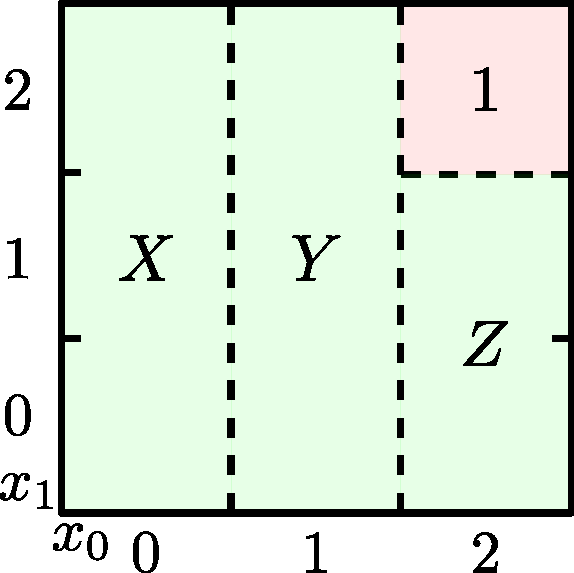
\includegraphics[scale=0.45]{figs/pd_split_thermal.pdf}
    \caption{\textbf{Qutrit phase space regions for $W_{\rho | \tau}(\x)$.}
    Here, the negative component of the magic state overlaps the Wigner distribution of $|0\>$. The rescaled distribution attains a single value in each of the four regions, proportional to the value depicted in the region, see~\cref{eq:bmw_rescaled}.
    }
    \label{fig:pd_split}
\end{figure}

We now denote by $\w(\rho), \w(\rho|\tau)$ the unique values occurring in $W_\rho(\x), W_{\rho|\tau}(\x)$ respectively and $\bmm$ the vector of associated multiplicities of each value in $W_\rho(\x)$. The component values and multiplicities of the relevant distributions in the four distinct regions are given by
\begin{align}
	\w(\rho) &\coloneqq (-v, u, u, u), \\
		\bmm &\coloneqq (1,2,3,3), \\
	\bmw(\tau) &\coloneqq \frac{1}{3\Z} \left( e^{-\beta E_0}, e^{-\beta E_0}, e^{-\beta E_1}, e^{-\beta E_2} \right), \\
	\bmw(\rho_{\rm{S}} | \tau) &\coloneqq 3\Z \left( -v e^{\beta E_0}, u e^{\beta E_0}, u e^{\beta E_1}, u e^{\beta E_2} \right). \label{eq:bmw_rescaled}
\end{align}

Using this notation, the values and multiplicities of the $n$--copy distribution $\bmw(\rho_n |\tau_n)$ are computed in~\cref{lem:ncopycomponents} in~\cref{app:cmpairs}. The values are given by 
\begin{align}\label{eq:ncopy_w_rescaled}
	[\w(\rho_n | \tau_n)]_{ijk} &= (3\Z)^{n} (-v)^{n-\alpha} u^{\alpha} e^{\beta (n-\alpha)E_s} e^{\beta ( i E_0 + j E_1 + k E_2 )},
\end{align}
where the indices $i,j,k$ are non-negative integers that obey the constraint $\alpha \coloneqq i+j+k \leq n$.
The multiplicity of this above value is $m_{ijk}$ with
\begin{equation}
	m_{ijk} = \frac{n!}{i!j!k!(n-\alpha)!} 2^i 3^j 3^k.
\end{equation}
The associated components of $\w(\rho_n)$ are given by
\begin{align}
	[\w(\rho_n)]_{ijk} &= (-v)^{n-\alpha} u^{\alpha}, \label{eq:ncopy_wrho}\\
	[\w(\tau)]_{ijk} &= (3\Z)^{-n} e^{-\beta (n-\alpha)E_s} e^{-\beta ( i E_0 + j E_1 + k E_2 )}. \label{eq:ncopy_wsigma}
\end{align}

In order to construct the $n$--copy Lorenz curve $L_{\rho_n|\tau_n}(x)$ we need to order the components of the distribution, $w(\rho_{\rm{S}} | \tau)_{ijk}$ in decreasing order, and identify the sequence of indices that give us $W_{\rho_n}(\pi(\x))$.

Generally this is complex, but in order to obtain distillation bounds it is sufficient to determine the location of the first elbow $(x_0, L_0)$ of $L_{\rho_n|\tau_n}(\x)$. To do so, we compute the largest component 
\begin{equation}
	w_{\rm max} \coloneqq \max_{i,j,k} [\w(\rho_n | \tau_n)]_{ijk},
\end{equation}
and determine the indices at which this occurs.
Putting in the values we obtain
\begin{align}
	&(3\Z)^{-n}w_{\rm max} = \nonumber\\
	&\max\limits_{i,j,k}\Big\{ (-v)^{n-\alpha} u^{\alpha} e^{\beta (n-\alpha)E_s} e^{\beta ( i E_0 + j E_1 + k E_2 )} \Big\}, \label{eq:max_slope}
\end{align}
where $0 \leq i,j,k \leq n$ and $\alpha \coloneqq i+j+k \leq n$.
Now for $0 \leq \epsilon \leq 3/7$, we have $v \geq u$. Since we assume that $n$ is even, we need the sum $\alpha = i+j+k$ to be even too, so that the expression is positive. 

Given an even value for $\alpha$, the term $v^{n-\alpha} u^{\alpha} e^{-\beta (n-\alpha)E_s}$ is fixed, so the expression is maximised by setting the coefficient of the highest energy $E_{\rm{max}}$ equal to $\alpha$.
Hence, we have
\begin{align}
	&w_{\rm max} = \nonumber\\
	&(3\Z)^{n} v^n e^{n\beta E_s}\max\limits_{\substack{\alpha = 0,2, \\ \dots,n-2,n}}{\Big\{ \left( \frac{u}{v} e^{\beta (E_{\rm{max}} - E_s)} \right)^{\alpha} \Big\}}.
\end{align}
If the expression $\frac{u(\epsilon)}{v(\epsilon)} e^{\beta (E_{\rm{max}} - E_s)}$ is less than $1$ then the maximum occurs at $\alpha=0$, otherwise it occurs at $\alpha = n$. For a fixed state $\tau$, this transition is determined by the value of the depolarising noise parameter $\epsilon$ of the noisy magic state. The transition occurs at $\epsilon = \epsilon_\star$ where
\begin{equation}\label{eq:noise_transition}
	\frac{u(\epsilon_\star)}{v(\epsilon_\star)} e^{\beta (E_{\rm{max}} - E_s)} = \frac{3-\epsilon_\star}{6-8\epsilon_\star} e^{\beta (E_{\rm{max}} - E_s)} = 1.
\end{equation}
If $E_{\rm{max}} = E_s$, namely if the state negativity lies in the same phase space region as the highest energy, this threshold is constant in temperature and given by $\epsilon_{\star} = 3/7$. However, the condition that $\epsilon_\star \ge 0$ also implies a constraint on the effective temperature of the stabilizer state. Specifically, there is a threshold temperature value $\beta_\star$ given by
\begin{equation}
	\beta_{\star} \coloneqq \frac{1}{E_{\rm{max}} - E_s} \ln2,
\end{equation}
such that for the regime $0 \leq \beta \leq \beta_\star$ a transition noise level $\epsilon_\star$ exists, and for $\beta > \beta_\star$ no such transition exists, so we choose $\epsilon_\star = 0$. 
Therefore, the transition value for the noise is given by
\begin{equation}
	\epsilon_{\star}(\beta) \coloneqq 
	\begin{cases}
		3 - \dfrac{9}{4-2^{\beta/\beta_\star - 1}}, &\text{ for } \beta \leq \beta_\star \\
		0, &\text{ for } \beta > \beta_\star.
	\end{cases}
\end{equation}
The quantity $w(\rho_{\rm{S}} | \sigma)_{\rm{max}}$ is now given by
\begin{equation*}
w_{\rm max} =
	\begin{cases}
		(3\Z)^{n} v^n e^{n\beta E_s}, &\mbox{if }\epsilon \leq \epsilon_{\star},\ \hspace{3pt}\rm{(C1)}\\
		(3\Z)^{n} u^n e^{n\beta E_{\rm{max}}}, &\mbox{if }\epsilon > \epsilon_{\star}.\ \hspace{5pt}\rm{(C2)} 
	\end{cases}
\end{equation*}
Case $\rm{(C1)}$ corresponds to $(i,j,k) = (0,0,0)$, so the multiplicity is $m_{000} = 1$, while
Case $\rm{(C2)}$ corresponds to
\begin{equation}
	(i,j,k) = 
	\begin{cases}
	(0,n,0), &\text{if } E_{\rm{max}} = E_1, \\
	(0,0,n), &\text{if } E_{\rm{max}} = E_2,
	\end{cases}
\end{equation}
so the multiplicity in both cases is $3^n$.

Using that $F = -\beta^{-1} \log \Z$, the first elbow coordinates in the two cases are now given by
\begin{equation}\label{eq:first_elb_coords}
	(x_0, L_0) =
	\begin{cases}
		\left(\frac{1}{3^n} e^{-n\beta (E_s - F)}, v^n \right), &\epsilon \leq \epsilon_\star \vspace{10pt}\\
		\left( e^{-n\beta (E_{\rm{max}}-F)}, (3u)^n \right). &\epsilon > \epsilon_\star
	\end{cases}
\end{equation}

\ddd{[Hmmm this needs an additional assumption on the output state to re-run the same analysis. Very annoying.]}\nick{What additional assumption beyond that the output state can be written as a Gibbs state for some $H'$?}
Similarly, considering the output magic state with respect to state $\sigma'$, the image of equilibrium state $\sigma$ under the magic protocol, we get output Lorenz curve coordinates,
\begin{equation}\label{eq:transformed_first_elb_coords}
	(x'_0, L'_0) =
	\begin{cases}
		\left(\frac{1}{3^{n'}} e^{-n\beta (E'_s - F')}, v(\epsilon')^{n'} \right), &\epsilon' \leq \epsilon'_\star \vspace{10pt}\\
		\left( e^{-n'\beta (E'_{\rm{max}}\hspace{-2.5pt}-F')}, (3u(\epsilon'))^{n'} \right), &\epsilon' > \epsilon'_\star
	\end{cases}
\end{equation}
There are four combinations of coordinates, depending on the noise parameters $\epsilon, \epsilon'$ for the input and output states.
In each of these combinations, we simply use the first elbow constraint, as described in~\cref{app:elb_constraints}, which leads to the bounds in the statement of the theorem.
\end{proof}

%%%%%%%%%%%%%%%%%%%%%%%%%%%%%%%%%%%%%%%%

\newpage
\subsection{Free energy dependent magic distillation bounds}\label{free-energy-bound-proof}
Here we prove theorem \ref{thm:free-energy}, which bounds magic distillation rates in terms of free energies.


\begin{theorem}
	Consider a magic distillation protocol on qutrits that transforms $n$ copies of an $\epsilon$--noisy Strange state into $m$ copies of an $\epsilon'$--noisy Strange state, with depolarising errors $\epsilon' \leq \epsilon \leq 3/7$. 
	
	Let $T =(k\beta)^{-1}$ be any temperature for the physical system and let $H= \sum_{k \in \mathbb{Z}_3} E_k |E_k\>\<E_k|$ be the Hamiltonian of each qutrit subsystem in its eigen-decomposition.
Assume that for $n,m \rightarrow \infty$ the protocol's channel generates negligible correlations on the equilibrium state $\tau$, and so $\tau^{\otimes n} \longrightarrow \tau^{\prime \otimes m}$ for $n,m \gg 1$. We write the state $\tau'$ as $\tau' = e^{-\beta H'}/\Z'$ for some Hermitian $H'$.

Given this, there are local Clifford changes of basis $C_1,C_2$, such that $\rho_1 := C_1 \rho_S(\epsilon) C_1^\dagger$ and $\rho_2 := C_2 \rho_S(\epsilon') C_2^\dagger$ for which the protocol gives
\begin{equation}
\rho_1^{\otimes n} \longrightarrow \rho_2^{ \otimes m}.
\end{equation}
Moreover, the magic distillation rate $R = m/n$ for the protocol is bounded by the expression
\begin{equation}\label{eq:rate_bounds_proof}
	R \leq \dfrac{\ln{\big( 1-\frac{4}{3}\epsilon \big)} + \beta (\phi - F)}{\ln{\big( 1-\frac{4}{3}\epsilon' \big)} + \beta (\phi' - F')},
\end{equation}
where $F$ is the free energy of $\tau$,  and 
\begin{equation}
\phi = -\beta^{-1} \log \zeta
\end{equation}
with $\zeta$ given by the equations
\begin{align}
\zeta &= \sum_{k\in \mathbb{Z}_3} \alpha_k e^{-\beta E_k}, \nonumber\\
\alpha_k &= \sum_{r \in \mathbb{Z}_3} \braket{E_k}{-r}\braket{r}{E_k}.
\end{align}
The primed variables are defined similarly for the output system.
\end{theorem}


\begin{proof}	
For the sake of clarity, we write $\rho_n \coloneqq \rho_S(\epsilon)^{\otimes n}$, $\rho'_m \coloneqq \rho_S(\epsilon')^{\otimes m}$, $\tau_n \coloneqq \tau^{\otimes m}$ and $\sigma_m \coloneqq \sigma^{\otimes m}$. 

To establish the distillation bound we consider the distillation protocol that gives $\E( \rho_n) = \rho_m$ for the magic states. 
We then consider that the protocol transforms the reference equilibrium state as $\E( \tau_n) = \sigma_m$.
Since $\tau$ and $\sigma$ are assumed to be full rank stabilizer states, they have a strictly positive Wigner distribution, while, in contrast, the input and output magic states generally have quasi-probability Wigner distributions. 
For any such protocol we therefore have that
\begin{equation}
	( W_{\rho_n}(\bmx), W_{\tau_n}(\bmx) ) \succ ( W_{\rho'_m}(\bmx), W_{\sigma_m}(\bmx) ),
\end{equation}
or, equivalently, in terms of the relevant Lorenz curves,
\begin{equation}
	L_{\rho_n |\tau_n}(x) \ge L_{\rho'_m |\sigma_m}(x) \mbox{ for all } x.
\end{equation}

We define the rescaled Wigner distribution $W_{\rho | \tau}(\x) \coloneqq W_\rho(\x)/W_\tau(\x)$, which is always well-defined since $\tau$ is full-rank. 
Due to the multiplicative property of the Wigner distribution, the rescaled distribution is also multiplicative in the sense that
\begin{equation}
	W_{\rho \otimes \rho' | \tau \otimes \tau'} (\x_1 \oplus \x_2) = W_{\rho | \tau}(\x_1)W_{\rho' | \tau'}(\x_2),
\end{equation}
for any states $\rho, \rho'$ and any full-rank stabilizer states $\tau, \tau'$.
Therefore we have that
\begin{align}
	W_{\rho_n |\tau_n} (\x) &= \prod_{i=1}^n W_{\rho|\tau}(\x_i)\\
	W_{\rho_n } (\x) &= \prod_{i=1}^n W_\rho(\x_i)
\end{align}
where $\x = \oplus_{i=1}^n \x_i \in \mathbb{Z}_3^n$ is the phase space point for the full system in terms of those of the individual subsystems.

The points defining the Lorenz curve $L_{\rho_n |\tau_n}(x)$ are obtained from sorting the components of $W_{\rho_n |\tau_n}(\x)$ in non-increasing order and then computing the partial sums of $W_{\rho_n |\tau_n}(\pi(\x))$ where $\pi$ is the permutation that realises the sorting. 
However, similarly to the unital fragment analysis, we aim to use the constraint that is obtained by considering the line segment connecting the origin to the first elbow of both Lorenz curves.
The proof of this constraint is provided in~\cref{app:elb_constraints}.
Therefore, we focus on finding the coordinates of some point on this line segment of the Lorenz curves.

We find the coordinates for the input Lorenz curve, but the exact same analysis can be applied on the output Lorenz curve.
The Wigner distribution of a single noisy Strange state consists of 1 negative component $W_{\rho}(0,0) = -v(\epsilon)$ and 8 positive components $W_{\rho}(\bmx) = u(\epsilon)$ for $\bmx \neq \bmo$.
The Wigner distribution of the full-rank, stabilizer equilibrium state $\tau$ is $W_{\tau}(\bmx) > 0$ for all $\bmx \in \mathbb{Z}_3^2$.
We keep the components completely general.

Assume that the smallest component of the equilibrium state distribution is $W_{\tau}(i,j)$.
We then make use of the freedom to apply Clifford unitaries in order to perform the  Clifford operation
\begin{equation}
	\tau \longrightarrow X^{-i}Z^{-j}\ \tau\ Z^{j}X^{i},
\end{equation}
which permutes the smallest component to the origin of the phase space, $W_{\tau}(i,j) \longrightarrow W_{\tau}(0,0)$.
This operation would inevitably affect the magic distillation protocol, but since we consider the state distillation modulo Clifford operations, we are allowed to perform the reverse Clifford operation keeping the magic distillation process as is. \nick{statement here is inaccurate}

The rescaled distribution components are in general given by
\begin{equation}
	W_{\rho_n|\tau_n} = \left(\frac{-v}{W_{\tau}(0,0)}\right)^{i_{\bmo}} \prod_{\bmx \neq \bmo} \left(\frac{u}{W_{\tau}(\bmx)}\right)^{i_{\bmx}},
\end{equation}
where the (integer) indices obey the following conditions:
\begin{align}
&0 \leq i_{\bmx} \leq n \mbox{ for all } \bmx \in \mathbb{Z}_3^2, \nonumber \\
&\sum_{\bmx \in \mathbb{Z}_3^2} i_{\bmx} = n.
\end{align}
It is now easy to find the largest rescaled component.
Firstly, note that $n$ is even, so we require that $i_{\bmo} \in \{0,2,\dots,n\}$ for the component to be positive.
Then, we have that $v \geq u$ because $\epsilon \leq 3/7$, and we have already ensured that $W_{\tau}(0,0) \leq W_{\tau}(\bmx)$ for all $\bmx \in \mathbb{Z}_3^2$.
Therefore, the largest rescaled component occurs when $i_{\bmo} = n$ and $i_{\bmx} = 0$ for $\bmx \neq \bmo$ and is equal to $(v/W_{\tau}(0,0))^n$.
Accordingly, the coordinates of the first Lorenz curve point after the origin are given by
\begin{equation}
	(x_0, L_0) = ((W_{\tau}(0,0))^n, v^n)
\end{equation}

Given a Hamiltonian decomposition,
\begin{equation}
	H = \sum_{k \in \mathbb{Z}_3} E_k\ketbra{E_k}{E_k},
\end{equation}
we can re-express the coordinate location, by writing
\begin{align}
	W_{\tau}(0,0) &= \frac{1}{3\Z}\tr\left[ A_{0,0}e^{\beta H} \right] \nonumber\\
	&= \frac{e^{\beta F}}{3} \tr\left[ \sum_{r \in \mathbb{Z}_3} \ketbra{-r}{r}\sum_{k \in \mathbb{Z}_3} e^{\beta E_k}\ketbra{E_k}{E_k} \right] \\
	&= \frac{e^{\beta F}}{3} \sum_{r \in \mathbb{Z}_3} \alpha_k e^{\beta E_k}
	= \frac{e^{\beta F}}{3} \zeta \\
	&= \frac{e^{\beta (F - \phi)}}{3},
\end{align}
where $\alpha_k, \zeta$ and $\phi$ are as defined prior to the statement of the theorem.
Finally, the coordinates can be expressed as
\begin{equation}
	(x_0, L_0) = \left( \frac{e^{n\beta (F - \phi)}}{3^n}, v(\epsilon)^n \right).
\end{equation}
In the same manner, we can derive the first point coordinates of the output Lorenz curve as
\begin{equation}
	(x'_0, L'_0) = \left( \frac{e^{n\beta (F' - \phi')}}{3^n}, v(\epsilon')^n \right).
\end{equation}

If the largest rescaled component of a state is distinct with no multiplicities, then these coordinates correspond to the first elbow of the corresponding Lorenz curve, whereas if it appears multiple times, then the coordinates derived correspond to a point on the interior of the line segment connecting the origin to the first elbow.
In both cases, the distillation bound remains the same, as is clear by its derivation in~\cref{app:elb_constraints}, and it is given by $L_0 / x_0 \geq L'_0 / x'_0$, which can be directly rearranged into the stated bound of the theorem.
\end{proof}



























